%%%%%%%%%%%%%%%%%%%%%%%%%%%%%% -*- Mode: Latex -*- %%%%%%%%%%%%%%%%%%%%%%%%%%%%
%% nsf.tex         : 2009 Smart Consumer Proposal
%% Author          : Philip Johnson
%% Created On      : Tue Mar 31 11:16:58 2009
%% Last Modified By: Philip Johnson
%% Last Modified On: Wed Dec 16 14:07:41 2009
%%%%%%%%%%%%%%%%%%%%%%%%%%%%%%%%%%%%%%%%%%%%%%%%%%%%%%%%%%%%%%%%%%%%%%%%%%%%%%%
%%   Copyright (C) 2009 
%%%%%%%%%%%%%%%%%%%%%%%%%%%%%%%%%%%%%%%%%%%%%%%%%%%%%%%%%%%%%%%%%%%%%%%%%%%%%%%
%% 
 
\documentclass{proposalnsf}
\usepackage[final]{graphicx}

% NSF proposal generation template style file.
% based on latex stylefiles  written by Stefan Llewellyn Smith and
% Sarah Gille, with contributions from other collaborators.

\renewcommand{\refname}{\centerline{References cited}}

% Fix things so that figures tend to stay away from the last page. 
\renewcommand{\topfraction}{0.85}
\renewcommand{\textfraction}{0.1}
\renewcommand{\floatpagefraction}{0.75}

% this handles hanging indents for publications
\def\rrr#1\\{\par
\medskip\hbox{\vbox{\parindent=2em\hsize=6.12in
\hangindent=4em\hangafter=1#1}}}

\def\baselinestretch{1}

%% URLs
\usepackage{url}
\usepackage[colorlinks, bookmarks=true]{hyperref}
\usepackage{breakurl}

\usepackage{floatflt}


\begin{document}

\newpage
%\pagenumbering{arabic}
%\renewcommand{\thepage} {C--\arabic{page}}
%\renewcommand{\thesection} {C.\arabic{section}}
\setcounter{section}{0}

%%%%%%%%%%%%%%%%%%%%%%%%%%%%%% -*- Mode: Latex -*- %%%%%%%%%%%%%%%%%%%%%%%%%%%%
%% project-background.tex -- 
%% Author          : Philip Johnson
%% Created On      : Tue Mar 31 11:44:58 2009
%% Last Modified By: Philip Johnson
%% Last Modified On: Wed Dec 16 15:29:18 2009
%% RCS: $Id$
%%%%%%%%%%%%%%%%%%%%%%%%%%%%%%%%%%%%%%%%%%%%%%%%%%%%%%%%%%%%%%%%%%%%%%%%%%%%%%%
%%   Copyright (C) 2009 
%%%%%%%%%%%%%%%%%%%%%%%%%%%%%%%%%%%%%%%%%%%%%%%%%%%%%%%%%%%%%%%%%%%%%%%%%%%%%%%
%% 

\section{Vision Statement}
\label{sec:vision}

% Enabling active participation in the Smart Grid through Open Power Quality.

% {\em The project description of a Type 1 proposal must begin with a concise statement of the project vision, situating an integrative, collaborative research project within a clearly articulated context of larger sustainability goals. It is understood that the proposed research may focus only on a piece of this vision, but the relationship of the proposed research to the overall vision must be articulated here. The vision statement must also briefly address important human, social, behavioral, economic, and adoption issues that are relevant, whether or not they are directly addressed within the proposed research.}

Development of the ``Smart Grid'', a modernized power infrastructure, is a key sustainability challenge facing the United States. According to the Department of Energy, the Smart Grid should: (1) Enable active participation by consumers by providing choices and incentives to modify electricity purchasing patterns and behavior; (2) Accommodate all generation and storage options, including wind and solar power.  (3) Enable new products, services, and markets through a flexible market providing cost-benefit trade-offs to consumers and market participants; (4) Provide reliable power that is relatively interruption-free; (5) Optimize asset utilization and maximize operational efficiency; (6) Provide the ability to self-heal by anticipating and responding to system disturbances; (7) Resist attacks on physical infrastructure by natural disasters and attacks on cyber-structure by malware and hackers \cite{NETL:GridCharacteristics}.

The very first goal, enable active participation by consumers, involves a fundamental paradigm shift.
Electrical utilities traditionally focus on achieving the opposite goal: enabling {\em passive} 
consumers whose participation is limited to plugging in appliances and paying a monthly bill. The historical success of utilities at reliably providing high quality power at low cost has led to multiple generations of consumers who need to know almost nothing about how their homes and workplaces are powered.

Initial efforts to enable active participation have focused on providing consumers with new forms of data regarding their energy consumption, and have achieved only moderate success.  Feedback on consumption does facilitate one-time positive behaviors, such as installing new insulation or purchasing energy efficient appliances. While helpful, such behaviors do not constitute active participation.    Time-of-use pricing is another approach to active participation, but the typical result is installation of controllers and a ``set it and forget it'' behavior.  Unfortunately, feedback on consumption can even facilitate negative behaviors, such as when consumers install grid-tied solar panels and then consume more electricity because it now appears to be ``free''.  In all of these approaches, consumer behavior is individual and independent of others. 

We propose a different path to active participation by consumers in the Smart Grid.  Based upon our experiences as consumers and energy researchers in Hawaii, we have found that high penetration of distributed, intermittent renewables such as rooftop photovoltaics has the potential for negative impact on power quality and overall grid stability \cite{Rodriguez2010,Laskar2012}, and that this potential negative impact has created actual technical, economic, and social problems in Hawaii.  On a technical level, we have observed power quality events at a weekly frequency in one of our households over the past year. On social and economic levels, our electrical utility has sought rate increases to improve infrastructure and limitations on the penetration of residential PV at the circuit level. Both of these actions have produced significant negative reactions from consumers, the media, and the government. 

One possible solution for Hawaii involves a much deeper level of active participation by consumers, in which we as a community take more direct interest in the state of our grid and more political and economic responsibility for its stability.  This is a tall order: how do we get there?

Over the past year, we have initiated the Open Power Quality (OPQ) research project, which involves designing and implementing a combination of low-cost hardware and cloud-based software that enables consumers to monitor the quality (voltage and frequency) of power in their household and upload that data to our Internet service in order to produce a crowdsourced perspective on grid health.  If effectively deployed, the data could enable consumers to learn for themselves whether their household is experiencing degraded power quality, whether this problem is isolated to their own house or widespread in their community, whether the problem is intermittent or frequent, and whether the problem is unpredictable or regularly occurring. The OPQ approach also has potential to support limited forms of prediction (such as whether certain forms of cloud cover create local instabilities) along with limited forms of diagnosis (such as whether an instability was a result of malfunction within a house or due to interactions between multiple houses).   In contrast to consumption-based approaches with their individually-oriented, one-off results, our quality-based approach has the potential to produce community-level engagement and policy-level activism.  

To test whether these potential benefits of crowdsourced power quality data can be achieved in practice, we propose a two year project to gather evidence regarding the following research questions:

\begin{enumerate}

\item {\em Can crowdsourced power quality data enable active participation in the Smart Grid?}

\item {\em What are the hardware, software, and analytic requirements for crowdsourced data that make it effective for prediction and diagnosis of Smart Grid power quality issues?}

\end{enumerate}

To investigate the first question, we will manufacture and distribute 300 power quality monitoring devices to volunteer households in three Oahu neighborhoods (selected to study low, moderate, and high penetration of distributed renewables). Through pre and post test questionnaires augmented with selected face-to-face interviews, we will assess the extent to which crowdsourced power quality data influenced 
consumer attitudes toward the electrical utility and public policy regarding the grid, as well as behaviors including interaction with neighbors regarding power quality and installation of appliance or whole house battery systems to improve household power quality.

To investigate the second question, we will augment the power quality data collected above with environmental data (temperature, humidity, wind speed and direction, and insolation), household consumption data (as available through an opt-in procedure), and household generation through photovoltaics (again, as available through an opt-in procedure).  We will perform exploratory analytics on the resulting dataset in an attempt to determine the necessary sampling rates, granularity, and history for local power quality, consumption, generation, and environment necessary to support prediction and/or diagnosis of power quality and grid stability. 

To be successful, our approach requires a combination of engineering, human-computer interaction, data analytics, and social science experimentation.  Our research team combines expertise from all of these disciplines. 

To maximize its benefits to and impact upon the scientific community, the OPQ project is ``triple open source'': the hardware schematics are available under the CERN Open Hardware License, the software and firmware are available under the GNU Public License Version 3, and (with consumer consent) the data collected will be available under the Open Data Commons Open Database License.  Our goal is to create an ecosystem of hardware, software, and data that maximizes progress in understanding grid dynamics and consumer involvement. 

As a longer range goal, we intend the OPQ project to provide a basis for research into the application of crowdsourced data to address other sustainability-related resources.  For example, water quality and air quality could be investigated using the same basic paradigm. 

In the remainder of this proposal we will review research related to Open Power Quality, present our project plan, and summarize its intellectual merit and broader impacts.


% Unfortunately, our current fossil fuel-based grid system is unsustainable for a variety of ecological, political, economic, and social reasons, and so a principle goal for the Smart Grid is to integrate distributed, intermittent energy sources such as wind and solar.  Hawaii, due to its high cost of energy, abundant availability of wind and solar, and small population, has become a living laboratory for the social, technical, and political problems that can occur during the transformation to a Smart Grid.

% For example, over the past five years, Hawaii has far exceeded the rest of the nation in the rate of installation of photovoltaics, and now has the highest per capita penetration of PV in the country.  This rapid uptake has been driven by economics: the combination of high electricity rates (roughly triple the mainland) coupled with tax incentives has meant that solar system installation costs can be recovered in 5-7 years. In Hawaii, companies will literally rent your roof to install panels. 
 
% Our recent experience in Hawaii shows that the goal of ``active participation'' is only partially, and sometimes just temporarily, achieved by consumers installing solar panels.  In fact, PV installation can actually work against this goal when consumers decide that the installation of solar panels has ``solved their energy problem'' and thus they no longer need to engage with the energy issue.   Worse, solar installation can increase consumptive behaviors (for example, running air conditioners more frequently or setting thermostats to a more consumptive setting) because PV owners now perceive their electrical energy as ``free''. 

% Hawaii's recent experience yields a great deal of insight into the social, technical, and economic complexities of achieving the various goals for the Smart Grid.  High penetration of a distributed, intermittent, and unpredictable energy source such as PV creates significant new challenges in maintaining grid reliability.  For example, on the island of Oahu, substations currently interpret backflow (i.e. energy flowing the ``wrong way'') as a fault in the grid, and respond by shutting down power distribution. This technical characteristic means that utilities must limit the installation of grid-tied PV below the substation level to an amount whose generation capacity does not exceed the lowest consumption level for the consumers serviced by that substation. Otherwise, the possibility exists that PV generation could exceed consumption, leading to backflow, interpreted as a fault, and subsequent shutdown. 

% This technical issue has had enormous social consequences. 

% Go from here into our hypothesis: that to get active participation, we need to not focus on consumption, which is an individual issue, but rather focus on energy quality, which is a community problem.   That if we can succeed in getting broad consumer engagement with the issue of power quality, then instead of ``withdrawing''  from the grid upon installation of PV, they will be more engaged as they realize that they are now partners with the utilities not only for generation but for reliability as well.  

% So, we will test this through the open power quality project....

% If successful, OPQ will have other benefits: the ability to create low-cost devices that will correlate grid power quality measurements with other factors. 

% (Have Leon Roose read this prior to submission.  Co-PIs?)



%%%%%%%%%%%%%%%%%%%%%%%%%%%%%%% -*- Mode: Latex -*- %%%%%%%%%%%%%%%%%%%%%%%%%%%%
%% project-background.tex -- 
%% Author          : Philip Johnson
%% Created On      : Tue Mar 31 11:44:58 2009
%% Last Modified By: Philip Johnson
%% Last Modified On: Wed Dec 16 15:29:18 2009
%% RCS: $Id$
%%%%%%%%%%%%%%%%%%%%%%%%%%%%%%%%%%%%%%%%%%%%%%%%%%%%%%%%%%%%%%%%%%%%%%%%%%%%%%%
%%   Copyright (C) 2009 
%%%%%%%%%%%%%%%%%%%%%%%%%%%%%%%%%%%%%%%%%%%%%%%%%%%%%%%%%%%%%%%%%%%%%%%%%%%%%%%
%% 

\section{Background and significance}

% {\em The proposal must provide adequate background for reviewers to judge the novelty, uniqueness, and significance of the proposed research.}

The OPQ research project involves the development of three basic components: power quality monitoring hardware, crowdsourced power quality data, and analytics to make the collected data useful. 

\subsection{Power quality monitoring hardware}
\label{sec:background-hardware}

There is wide variety in the capability, cost, and user community for power quality monitoring devices.

Starting at the high end, a phasor measurement unit (PMU) captures measurements of voltage or current at a rate of 30-60 Hz, and uses GPS to ensure that the timestamps recorded between different PMUs are accurate to approximately 1 microsecond \cite{Zhang2007}. As of 2010, there were approximately 200 installed PMUs in the North American power grid. The cost of a single PMU hardware device and its installation on a transmission line can reach \$100,000. The PMU user community consists of utilities who install and maintain PMUs at substations or generation plants in order to assess grid stability.

The Wide-Area Frequency Monitoring Network (FNET) is a project by researchers at Virginia Tech based upon a GPS-synchronized single-phase ``frequency disturbance recorder'' (FDR) that can be installed at ordinary 120V outlets \cite{Zhang2010}. Currently, FNET gathers frequency and voltage data from approximately 80 FDRs installed across North America.  By monitoring changes, FNET can detect generator trips (which cause a decline in frequency) and load shedding (which cause an increase in frequency). Because the geographical location of each FDR is known, and because the timestamps are synchronized to less than a microsecond, FNET can be used to triangulate both the original size and location of such events. The FNET user community is a consortium consisting of utilities, power companies, and government groups.  The cost of an FDR is \$2500.

% In summary, PMUs and FDRs are both wide-area, distributed devices for monitoring power quality at the grid-level through highly synchronized, time-stamped data. PMUs monitor voltage and current, while FDRs monitor frequency and voltage.  Both 
% user communities are utilities and large power technology companies. 

Industrial manufacturing companies form a different user community for power quality monitoring. These companies are not concerned with overall grid quality but only with the quality of the power received at their buildings.  For example, devices such as PQube \cite{pqube} connect to AC power and can collect a variety of power data including voltage, frequency, THD, and VARs. PQube data is highly accurate and each device comes with an NIST calibration certificate. A single PQube device can cost over \$5,000.  Companies such as Fluke, PowerSight, and Tektronix also sell devices for measuring power quality problems in industrial or laboratory settings, for prices generally starting around \$1,000.

A partnership consisting of the California Institute for Energy and the Environment, Power Standards Lab, Lawrence Berkeley National Lab, and UC Berkeley are extending PQubes with custom hardware to create ``micro'' PMUs \cite{Meier2013,Meier2014}.  The goal is to manufacture PMUs at a low enough price point to justify their installation below the transmission level, and thus provide utilities with additional data that improves their situational awareness and faster service restoration.  

Residential consumers form a relatively unexplored user community for power quality monitoring.   One of the few commercial products for this user community is the AC Scout \cite{acscout}.  This device plugs into 120V power outlets and can monitor voltage and frequency.  Depending upon the model, the AC Scout costs between \$200 and \$400. The AC Scout is designed only to monitor a single household, and is designed to write entries to a log file when pre-defined thresholds for voltage and frequency are exceeded. The log file can be off-loaded from the device to a computer via a USB cable or sent via email if the ethernet cable connection to the Internet is provided. Since data from one AC Scout is not intended for comparison with others, there is no attempt at synchronization.

\begin{figure}[h]
  \begin{tabular}{l|r|p{2in}|p{1in}|p{1in}} \hline
  {\bf Device} & {\bf Cost} & {\bf Measurements} & {\bf Synchronization} & {\bf Communication} \\ 
  PMU & \$100,000 & frequency, voltage, current & GPS & Secure LAN  \\
  FDR & \$2,500 & frequency, voltage & GPS & Internet \\
  PQube & \$5,000+ & frequency, voltage, THD, VARs & (none) & (none)  \\
  mPMU & \$5,000+ & frequency, voltage, THD, VARs & GPS & Custom network \\
  AC Scout & \$200+  & frequency, voltage & (none) & (none) \\
  OPQ & \$60 & frequency, voltage, THD & NTP & HTTP/SSE \\
  \hline
  \end{tabular}
  \caption{\em \small Comparison of hardware devices for power quality monitoring}
  \label{fig:hardware-table}
\end{figure} 

Figure \ref{fig:hardware-table} summarizes how the OPQ quality monitoring hardware contrasts with the above devices. First, we will monitor total harmonic distortion in addition to frequency and voltage, and we will also store waveform data for the past 24 hours in order to explore the possibility of diagnosis when thresholds are exceeded.  Second, we expect to be able to produce the devices for approximately \$60, a price point similar to conventional power strips with surge protectors, and significantly less expensive than any power quality monitoring device of which we are aware. Third, our devices will use WiFi for communication with our cloud-based service via HTTP and Server-Sent Events protocols.  Fourth, our devices will use Network Time Protocol (NTP) for synchronization.  While GPS-based synchronization provides an accuracy below a single microsecond, NTP-based synchronization provides a much lower accuracy of a few milliseconds. Use of NTP limits the kinds of analytics that can be performed with OPQ, but reduces both the cost and constraints upon installation location. The impact of this trade-off will be assessed as part of this research. 

\subsection{Crowdsourced power quality data}

Up to now, geographically distributed power quality data has been collected by and oriented toward the needs of utilities. The OPQ project proposes an alternative, crowdsourced approach, in which collection is by and analysis is oriented toward the needs of consumers.   

According to Estelles-Aroles, crowdsourcing is ``a type of participative online activity in which an individual, an institution, a non-profit organization, or company proposes to a group of individuals of varying knowledge, heterogeneity, and number, via a flexible open call, the voluntary undertaking of a task. The undertaking of the task [...] always entails mutual benefit. The user will receive the satisfaction of a given type of need, be it economic, social recognition, self-esteem, or the development of individual skills, while the crowdsourcer will obtain and utilize to their advantage that what the user has brought to the venture, whose form will depend on the type of activity undertaken.'' \cite{Estelles-Aroles2012}.

To our knowledge, crowdsourcing has never been successfully used for the purpose of collecting and analyzing power quality data.  That said, Hammack proposed this very idea as ``citizen engineering'' in 2010, suggesting that the deployment of several thousand FNET frequency disturbance devices could be combined with publicly accessable online tools for visualization and analytics to enable consumers to see how their frequency data relates to that of the rest of the nation \cite{Hammack2010}.   We believe his idea did not gain traction due to the cost of the devices and the relatively low benefits to individuals of a nation-wide perspective on frequency changes.  In contrast, the OPQ project is designed to address both of these issues by the design of less expensive devices, and the deployment into a geographically small user community that is actively ``suffering'' from issues related to power quality.  

Privacy is an important issue when crowdsourcing data about individuals or their environment. One successful example of a crowdsourced project that has addressed this issue is the Personal Genome Project (PGP), in which individuals are asked to share their genetic data in order to create a public repository that can advance the science of health care \cite{Church2005}. PGP data is placed in the public domain and contributors are required to sign an ``open consent'' form which states that the researchers cannot guarantee anonymity. In the OPQ project, we address privacy by allowing contributors to ``coarsen'' the published geographical location of their power quality data in order to address privacy concerns.  The adequacy of this approach will be assessed as part of this research.

\subsection{Analytics}

Power quality data is traditionally used for four purposes: (1) {\em detection} of anomalies, (2) {\em diagnosis} of the cause and/or originating location of the anomaly, (3) real-time {\em control} of grid stability, and (4) {\em prediction} of future anomalies. Whether or not a given data set can be used for any of these purposes depends upon the characteristics of its generating device. A relatively simple device like the AC Scout can be used only for detection, FNET can be used for both detection and diagnosis \cite{Markham2012}, and PMU data can be applied to detection, diagnosis \cite{Zhao2009}, control \cite{Liu2010}, and prediction \cite{Liu2009,Gao2012}). 

The OPQ project is designed to collect power quality data that can be used for detection of anomalies and a limited form of diagnosis: if a user lives in a neighborhood where several OPQ devices are installed, then an anomaly report will indicate if it was limited to the users household or co-occurred elsewhere in the neighborhood. Our devices are not sufficiently synchronized, nor can the data be communicated to grid operators quickly enough to support real-time control. We will also investigate whether or not the data collected from our devices can support some forms of prediction when combined with other environmental, consumption, and generation data. From this traditional perspective on the use of power quality data, the OPQ project results in a data set that has somewhat more capability than the data collected from devices like the AC Scout, yet less capability than the data collected by devices like FDRs and PMUs. 

However, in addition to the four traditional purposes, the OPQ project is designed to investigate whether power quality data can be used for an entirely new purpose: (5) {\em enabling active participation by consumers}. To do this, we will develop some simple guidelines for interpretation of the data, helping consumers to decide if their problems are severe enough to contact the utilities or install UPS systems to protect sensitive equipment such as computers.  This makes power quality data {\em actionable}.

We observe that one cause of the societal and political issues involving the Smart Grid in Hawaii involves a fundamental disengagement by consumers from the grid: they want the utility to support unlimited installation of distributed generation by consumers (and resulting lower utility bills) without any perceivable impact on quality, price, or availability.  We hypothesize that a low-cost approach to providing consumers with increased visibility into grid stability can increase engagement (by enabling consumers to see how power quality varies from time to time and from neighborhood to neighborhood) followed by active participation (through policy and civic engagement) to create a Smart Grid satisfying everyone's needs.  Our project is designed to provide preliminary evidence regarding whether or not this fifth purpose can occur in reality.

In summary, our OPQ project will design and produce innovative hardware for power quality monitoring. We will implement an innovative, crowdsourced appoach to power quality data collection. Finally, we will apply this data to both traditional and entirely new purposes.   
%%%%%%%%%%%%%%%%%%%%%%%%%%%%%%% -*- Mode: Latex -*- %%%%%%%%%%%%%%%%%%%%%%%%%%%%
%% project-plan.tex -- 
%% Author          : Philip Johnson
%% Created On      : Tue Mar 31 11:44:58 2009
%% Last Modified By: Philip Johnson
%% Last Modified On: Wed Dec 16 15:29:18 2009
%% RCS: $Id$
%%%%%%%%%%%%%%%%%%%%%%%%%%%%%%%%%%%%%%%%%%%%%%%%%%%%%%%%%%%%%%%%%%%%%%%%%%%%%%%
%%   Copyright (C) 2009 
%%%%%%%%%%%%%%%%%%%%%%%%%%%%%%%%%%%%%%%%%%%%%%%%%%%%%%%%%%%%%%%%%%%%%%%%%%%%%%%
%% 

\section{Research plan}

% {\em The proposed research must approach fundamental research from an interdisciplinary perspective that integrates computing and communications with domain sciences and engineering to address the sustainability issues of interest. The proposal must describe a synergistic approach by which the team addresses scientific challenges in sustainability.}

Our research plan has three basic three phases: {\em Design and implementation}, {\em Deployment}, and {\em Assessment}.  The design and implementation phase will last approximately six months and will complete the hardware and software systems now under development. The deployment phase will follow the design and implementation phase and last approximately one year. Deployment involves the distribution of our hardware to three neighborhoods and collection of power quality data.  The assessment phase will begin in parallel with deployment and last one and a half years. During assessment we will collect evidence to answer the primary research questions presented in Section \ref{sec:vision}.

\subsection{Phase 1: Design and implementation}

The OPQ Project has been working on the design and implementation of open source hardware and software for the past year. In essence, our OPQ hardware device plugs into a normal 120V outlet, monitors frequency, voltage, and THD, and sends {\em events} via WiFi to our cloud-based software service when thresholds are exceeded.  Our OPQ cloud service gathers event data from devices and issues {\em alerts} to users via email or text message to inform them about power quality issues. Finally, our cloud service can send commands back to hardware devices, such as to change threshold values or retrieve recent waveform data for cloud-based analysis.

\subsubsection{OPQ Hardware Device}

Our OPQ hardware device has the following major design goals: (1) Unit price below \$60 to support large-scale deployment; (2) easy to install and safe to operate; (3) 16/24 bit resolution and 50+ samples per grid cycle; (4) Support for frequency voltage, and THD measurement; (5) onboard processing and local storage; (6) inter-device synchronization via NTP; (7) easy extensibility; and (8) open source license. 

\begin{wrapfigure}{r}{3.25in}
  \includegraphics[width=0.5\textwidth]{figures/hardware-block-diagram.eps}
  \caption{\em \small Hardware block diagram}
  \label{fig:hardware-block-diagram}
\end{wrapfigure} 

Figure \ref{fig:hardware-block-diagram} shows a block diagram and photo of the prototype hardware. In order to make our device safe to operate, it is galvanically isolated from the power grid via a UL-listed wall plug transformer. This transformer is used both for powering the meter and monitoring the power grid. The output of the transformer's secondary windings is passed through a low-pass filter which is responsible for scaling down the voltage to the analog-to-digital converter(ADC) range, as well as filtering out frequencies above 1Mhz. Furthermore this filter protects the sensitive inputs of the ADC.

The output of the filter is digitized using an ADC on an MSP430AFE microcontroller. This microcontroller is specifically designed for power metering. As illustrated in Figure \ref{fig:board}, we combine an analog front-end, a 24bit SAR ADC capable of sampling at 4kHz, and a 16bit MCU into a single integrated circuit to reduce the bill of materials. 

\begin{wrapfigure}{r}{0.35\textwidth}
  \includegraphics[width=0.35\textwidth]{figures/board3.eps}
  \caption{\em \small OPQ Board}
  \label{fig:board}
\end{wrapfigure} 

For our sensor network to scale, a significant amount of processing must be performed on the device itself. This includes power quality event detection, as well as buffering of historic data leading up to the event. Furthermore, event data needs to be uploaded to the cloud for further analysis. Currently, we use a Raspberry Pi single board computer for the main processing unit. The MSP430AFE sends digitized samples to the Raspberry Pi via the SPI protocol. Data is compared to the expected waveform, and if the deviation is significant, an event containing the raw data is send to the cloud via a USB 802.11 adapter. We have designed a custom protocol for data transmission to reduce the bandwidth required \cite{opq-protocol}. The device and cloud service communicate using server-side events (SSE) over HTTP, which enables the device to be sent commands from the cloud even though it will be located behind a home wireless router.

During this phase, we will hire a professional engineer experienced in this kind of product design to review our hardware for safety issues. 

\subsubsection{OPQ Cloud-based software service}

\begin{wrapfigure}{r}{3.25in}
  \includegraphics[width=0.5\textwidth]{figures/cloud-grid.eps}
  \caption{\em \small Cloud service page illustrating zoomable grid}
  \label{fig:cloud-grid}
\end{wrapfigure}  

In parallel with hardware, we have developed a cloudbased service for collection and analysis of the data. All source code is licensed under the GPL V3 and is available on GitHub \cite{opq-github}.  When a consumer receives a device, they use a browser to access our service and begin by completing a registration wizard. First, the wizard helps users to specify the kinds of alerts they want to receive and how they want to receive them (email or text message).  Users can specify both thresholds for event triggering, frequency of alert delivery (immediately, or as part of a daily or weekly summary), and whether they want to be alerted to only their own quality events or to quality events (and annotations of these events) in their neighborhood.  

Second, the wizard provides a privacy-preserving means to specify the location of the hardware device. It does this by presenting users with a map overlaid with zoomable tiles allowing them to select a location with resolutions from 500 square feet (typically revealing the actual building containing the device) to 1 square mile (revealing only the neighborhood containing the device). This is illustrated in Figure \ref{fig:cloud-grid}.

There are two addition forms of energy data that the user can choose to provide to the OPQ service through the wizard.  Some users may have PV and/or smart meters installed that provide internet access to consumption and/or generation data.  When available (and if the user is willing to share this data), the wizard will collect the information required to automatically retrieve this data as well.  Thus, in the best case, our service will have access to consumption, generation, and quality data about a single household.

After configuration, the service will push events to the user as specified in the user's preferences.  Beyond simple numerical data, the service can provide interpretation of the data, such as whether the frequency and/or severity of events is relatively low or high, and if high, actions that the user might want to consider.  These actions could include: (1) contacting the utility to request service (contact information supplied in the email); (2) Communicating with neighbors to see if they have power quality problems (via the creation of public annotations of their events); or (3) advice regarding ameliorative actions (such as installation of UPS line conditioning for sensitive appliances, if the frequency/severity of power quality problems appears to warrant this step.

\subsection{Phase 2: Deployment}

After the hardware is designed and a small pilot manufacturing run has established device quality, we will manufacture 150 units for trial deployment.  Although our current hardware design requires WiFi, the 2012 US Census Report indicates that 85\% of Hawaii households have internet access \cite{home-internet-access}, so we do not expect this to be a problematic constraint. 

Our deployment will begin by dividing the units among three Oahu neighborhoods based upon the penetration of photovoltaics on their associated circuit.  Our utility publishes a ``Locational Value Map'' indicating the penetration of PV on a daily basis \cite{lvm}, and we will use this to choose one neighborhood with low penetration (i.e. where PV comprises less than 50\% of the circuit's daytime minimum load), medium penetration (i.e. where PV comprises 75\% to 100\% of the circuit's daytime minimum load) and high penetration (i.e. where PV comprises 120\% or greater of the circuit's daytime minimum load). 

Within a single neighborhood, we will choose participants to receive devices in order to obtain households both with and without photovoltaics. We want to obtain variety in monthly electricity bills (small being below \$50, medium being between \$50 and \$150, and large being above \$150).  We hope at least 20\% of the households will opt-in to providing consumption and/or generation data in addition to power quality data. 

To facilitate deployment, we will request the aid of local environmental and sustainablity groups, including Kanu Hawaii, Blue Planet Foundation, and Kokua Foundation.  Hardware devices will be provided free of charge to participants, with their incentive for participation being increased access to information about their household power quality.  

Our devices will be installed with a unique ID that is sent with each communication to the cloud-based service to identify the originating device.  We can use this information to determine whether users have installed and configured the device successfully, and if a previously functioning device has ceased to transmit data.   In either of these cases, we will contact the user to see if they no longer wish to participate and if so, retrieve the device for redistribution. 

We plan to collect data during the Deployment phase for at least six months. However, if the deployment is proceeding successfully we will continue with data collection for up to 18 months (or the end of the grant period).  Further data collection at that point will depend upon the availability of funds for the cloud-based service.

During the course of deployment we will be accessing online NOAA weather data to collect environmental data (temperature, humidity, winds, insolation) for the neighborhoods selected for participation. 

In parallel with the deployment phase, we will begin the Assessment phase. 

\subsection{Phase 3: Assessment}

Assessment of this project will involve both qualitative (questionnaire) and quantitative (power quality) data, and is designed to provide insight into the two general research questions presented in Section \ref{sec:vision} as well as test several specific hypotheses described below. Our assessment procedure is as follows:

First, we will ask users to fill out a questionnaire when they receive their hardware device.  The questionnaire will assess their attitudes toward the electrical utility and the Smart Grid as well as their current electricity-related behaviors (i.e. recent electric bill amount indicating their consumption, presence of PV installation, use of hybrid or electric car). This will provide baseline information regarding attitude and behavior that we can use to assess the impact of access to power quality data.

Second, we will monitor the data over the course of deployment in order to ensure that hardware devices are being used, that they maintain high levels of uptime, and that power quality alerts are being observed and sent to users.  Based upon our experience with household installation of an AC Scout, we are confident that power quality problems will be observed in a significant fraction of the households.  In the event that a deployment does not generate a significant number of alerts in a given neighborhood after three months, we will manufacture additional devices and deploy to additional neighborhoods as necessary until we are able to obtain enough alerts to test our hypotheses.

Third, as soon as deployment begins, we will begin analysis of the collected power quality data to see if we can determine relationships with the environmental data we are also collecting. 

Fourth, upon conclusion of the deployment phase, we will ask users to fill out a second questionnaire.  This questionnaire will ask many of the same questions as the initial questionnaire, but will also ask if users made any changes with respect to their electrical behavior during the study period (such as installation of PV, installation of line conditioners, buying a hybrid vehicle, etc.) and to what extent these changes were motivated by information about their power quality.  This pre and post-test design will provide evidence regarding the ability of power quality data to enable active participation in the Smart Grid.  In addition to this self-reported data, we will also be able to observe ``active participation'' in the form of annotations users provide to their timeline.

Based upon analysis of the qualitative and quantitative data, we will test the following specific hypotheses: (1) Knowledge of personal power quality problems will lead to actions such as contacting the utilities or installing UPS line conditioners; (2) Intrinsic motivators (insight into personal and neighborhood power quality) suffice for participation in crowdsourced data collection; (3) Knowledge of neighborhood power quality issues will lead to active engagement with neighbors; (4) Recommendations provided by OPQ system will be found useful by users; (5) The frequency and severity of events will be positively correlated with the degree of penetration of distributed PV on that circuit.






















%%%%%%%%%%%%%%%%%%%%%%%%%%%%%%% -*- Mode: Latex -*- %%%%%%%%%%%%%%%%%%%%%%%%%%%%
%% project-background.tex -- 
%% Author          : Philip Johnson
%% Created On      : Tue Mar 31 11:44:58 2009
%% Last Modified By: Philip Johnson
%% Last Modified On: Wed Dec 16 15:29:18 2009
%% RCS: $Id$
%%%%%%%%%%%%%%%%%%%%%%%%%%%%%%%%%%%%%%%%%%%%%%%%%%%%%%%%%%%%%%%%%%%%%%%%%%%%%%%
%%   Copyright (C) 2009 
%%%%%%%%%%%%%%%%%%%%%%%%%%%%%%%%%%%%%%%%%%%%%%%%%%%%%%%%%%%%%%%%%%%%%%%%%%%%%%%
%% 

\section{Results from prior NSF support}

P. Johnson, {\em Human centered information integration for the Smart Grid}, NSF Grant IIS-1017126, 8/15/10 to 7/31/14, \$413,467. 
{\em Intellectual Merit:} The research provided novel insight into: the inadequacy of baseline data for energy competition research, the design of experimental studies for assessing energy behaviors, the design of energy competitions incorporating educational activities. 
{\em Broader Impacts} include: the creation and distribution of two open source systems, WattDepot and Makahiki, that can be used for collection and analysis of energy data and the design and implementation of sustainability games; the publication of data regarding the impact of energy
education and gamification techniques on energy literacy and behavior; the training of approximately 9 undergraduate students, 3 M.S. students, and 3 Ph.D. students in research techniques, sustainability concepts, and software design and development.
Selected publications:
  \cite{csdl2-10-05,csdl2-10-07,csdl2-10-08,csdl2-11-02,csdl2-11-03,csdl2-12-06,csdl2-11-07, csdl2-12-12,csdl2-13-10,csdl2-13-05,csdl2-13-03}. Research products are available at the Kukui Cup site \cite{kukuicup}, the WattDepot site \cite{wattdepot}, and the Makahiki site \cite{makahiki}.

A. Kuh and M. Fripp, {\em Sensing, Modeling, and Control of Smart Sustainable Microgrids}, NSF Grant ECCS-1310634, 7/1/2013-6/30/2016, \$360,000. 
{\em Intellectual Merit:} This project explores the potential of future power distribution by designing, building and evaluating a microgrid that offsets local energy usage using distributed generation (i.e. rooftop PV).
{\em Broader Impacts} include: By developing an operational structure analogous to the larger utility grid, the campus microgrid is being instrumented to serve as a platform for gathering field data on load, generation, local grid quality and usage patterning. Using this platform, students, faculty and partners can immediately advance their knowledge on the challenges of operating, monitoring and assessing the conditions of a modern grid. Selected publications: \cite{Fatemi2014}.

% \vspace{-.1in}

% \item A. Kuh, {\em Incremental and Distributed Learning in Nonstationary
%     Environments with Applications to Wind Forecasting}, NSF Grant ECCS-098344,
%   9/01/09 - 8/31/13, \$150,251.  The objective of this research is to
%   design novel nonlinear kernel online and distributed learning algorithms
%   for applications including wind forecasting.   Research was also conducted
%   to model the microgrid using a factor-graph framework. 
%   Selected publications for
%   this project include \cite{kuh-etal10,kowahl-kuh,hu-etal10,hu-kuh-yang-kavcic,hu-kuh-kavcic-nakafuji,ji-wei-kuh,uddin12,kuh-isess,carland,navid}.
  
% %\vspace{-.1in}

% \item A. Kuh, {\em US-Japan Joint Seminar Information Theory}, NSF Grant 0508025
%   \$35,750.  Funds used to support graduate students for conferences and
%   for visit to Japan.


%\vspace{-.1in}





%%%%%%%%%%%%%%%%%%%%%%%%%%%%%% -*- Mode: Latex -*- %%%%%%%%%%%%%%%%%%%%%%%%%%%%
%% biblio.tex -- 
%% Author          : Philip Johnson
%% Created On      : Fri Apr 03 14:56:50 2009
%% Last Modified By: Philip Johnson
%% Last Modified On: Thu Dec 10 10:44:01 2009
%% RCS: $Id$
%%%%%%%%%%%%%%%%%%%%%%%%%%%%%%%%%%%%%%%%%%%%%%%%%%%%%%%%%%%%%%%%%%%%%%%%%%%%%%%
%%   Copyright (C) 2009 
%%%%%%%%%%%%%%%%%%%%%%%%%%%%%%%%%%%%%%%%%%%%%%%%%%%%%%%%%%%%%%%%%%%%%%%%%%%%%%%
%% 

%\pagenumbering{arabic}
%\renewcommand{\thepage} {D--\arabic{page}}

\bibliography{smartconsumer,csdl-trs,ref-ak}
\bibliographystyle{plain}



\end{document}

